\begin{frame}
    \frametitle{Version Control}
    \begin{center}
        Version control is the practice of the tracking changes.
    \end{center}
\end{frame}

\begin{frame}
  \frametitle{Illustrative example: document states}
  Repository - the directory containing your project's code and files.
  \begin{figure}[htpb]
      \centering
      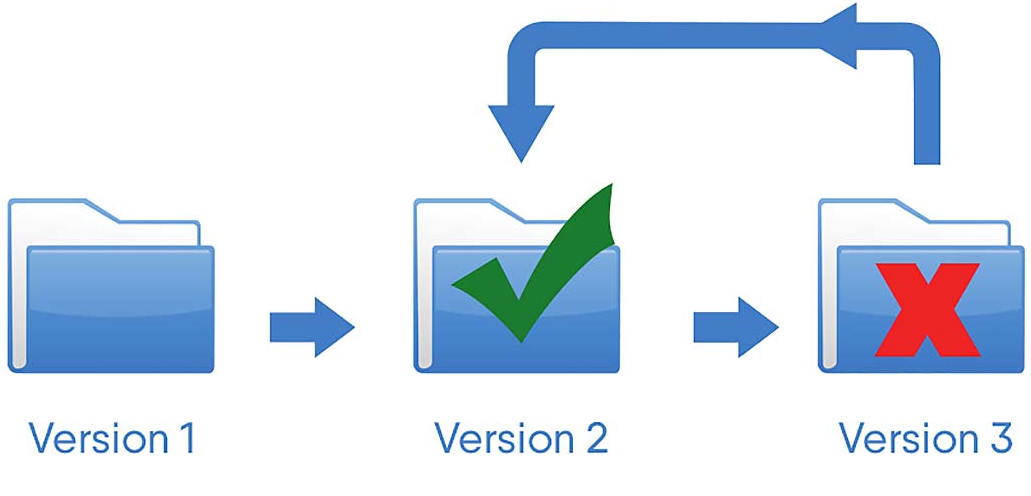
\includegraphics[width=0.8\textwidth]{images/singleton-vc.png}
  \end{figure}
\end{frame}

\begin{frame}
    \frametitle{Illustrative example: branching}
    \begin{itemize}
       \item Branch - a copy of the states of all the files in the project.
       \item Commit - a snapshot of changes of a specific group of staged files. Typically contain a {\it commit message} that describes the change.
    \end{itemize}

    \begin{figure}[htpb]
        \centering
        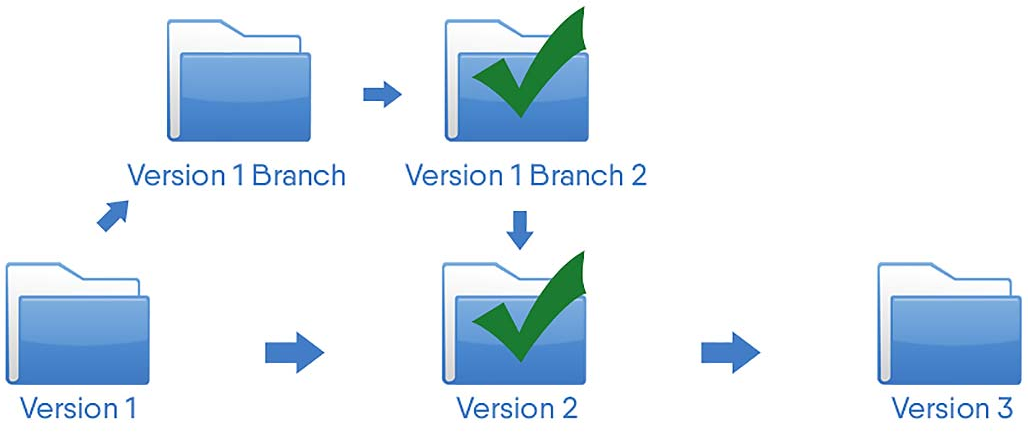
\includegraphics[width=0.8\textwidth]{images/branching-vc.png}
    \end{figure} 
\end{frame}

\begin{frame}
    \frametitle{Version Control Systems}
    \begin{figure}[htpb]
        \begin{subfigure}
        \centering
            
\includegraphics[width=2cm]{images/git-logo.eps}
        \end{subfigure}
        \begin{subfigure}
        \centering
            
\includegraphics[width=2cm]{images/mercurial-logo.eps}
        \end{subfigure}
        \begin{subfigure}
        \centering
            
\includegraphics[width=2cm]{images/subversion-logo.eps}
        \end{subfigure}
    \end{figure}
    \begin{center}
        {\tiny Sources: \cite{git_logo}, \cite{mercurial_logo}, \cite{subversion_logo}}
    \end{center}

    Software that tracks file states via commits.

    Basic workflow:
    \begin{enumerate}
        \item Make changes to tracked files in your local repository
        \item Stage the changes.
        \item Commit the stages changes to the repository
        \item Push the commited changes to a remote repository (where the official version of the code is hosted)
    \end{enumerate}
\end{frame}

\begin{frame}[fragile]
    \frametitle{A real-life \verb:git: example}
    \framesubtitle{Fixing a typo in OpenMC}

    Excerpt of \verb:openmc/surface.py: (lines 1970 - 1972)

    \definecolor{bg}{rgb}{0.95,0.95,0.95}
    \begin{minted}[bgcolor=bg]{python}
class ZCone(QuadricMixin, Surface):
    """A cone parallel to the x-axis of the form :math:`(x - x_0
    )^2 + (y - y_0)^2 = r^2 (z - z_0)^2`.
    \end{minted}
    Make our fix:
    
    \begin{minted}[bgcolor=bg,highlightlines={2}]{python}
class ZCone(QuadricMixin, Surface):
    """A cone parallel to the z-axis of the form :math:`(x - x_0
    )^2 + (y - y_0)^2 = r^2 (z - z_0)^2`.
    \end{minted}
\end{frame}

\begin{frame}[fragile]
    \frametitle{A real-life \verb:git: example}
    \framesubtitle{Fixing a typo in OpenMC}

    In the shell:
    \definecolor{bg}{rgb}{0.95,0.95,0.95}
    \begin{minted}[bgcolor=bg]{shell}
user@computer1:~/openmc$ git add openmc/surface.py
user@computer1:~/openmc$ git commit -m "fix axis spec in docstri
ng for ZCone"
user@computer1:~/openmc$ git push
    \end{minted}

    In this case, we pushed to the openmc-dev/openmc repository on GitHub. The commit is here $\rightarrow$ \url{https://github.com/openmc-dev/openmc/pull/2018/commits/48dbf1a4c3a83bf7abd0722ab868f532abc6b5bd} 
\end{frame}
